\documentclass[10pt,twocolumn]{article}
\usepackage[margin=0.75in]{geometry}
\usepackage[T1]{fontenc}
\usepackage{lmodern}
\usepackage{graphicx}
\usepackage{booktabs}
\usepackage{tikz}
\usepackage{amsmath}
\usepackage[hidelinks]{hyperref}
\usepackage{microtype}
\title{More Compliant, Less Aware:\\Diagnosing Post-Training Collapse in Multimodal Robot Failure Critics}
\author{Anonymous workshop submission}
\date{}
\begin{document}
\maketitle
\begin{abstract}
Can a robot execution critic become more compliant with its output protocol while losing the ability to recognize failure? We study this question using causal multi-view windows from REBOOT precision assembly and a Qwen2.5-VL-3B critic. In a retrospective six-episode discovery set, an exact-schema parser scores the Base model at zero because all 54 responses carry outer Markdown fences; a fixed mechanical fence-removal diagnostic instead recovers 54 valid responses and 6/18 failure windows. After supervised fine-tuning (SFT), strict JSON validity reaches 100\%, but failure recall falls to 0/18. Historical GRPO and exploratory GSPO runs also predict no failure, with recovery dominating their state distributions. These observations motivate, rather than establish, a mechanism claim: interface compliance, supervision density, camera observability, output-task coupling, and verifier reward must be disentangled. We define paired, episode-disjoint experiments and a failure-first RL gate. The internal Tier B final refit is in progress; no independent cross-task or causal reward-intervention result is claimed here.
\end{abstract}

\section{Introduction}
Robot policies can fail at contact-rich assembly without a clean binary boundary between success and failure. A monitor that returns syntactically valid output but misses the failure interval cannot reliably support recovery. REBOOT supplies phase- and failure-annotated bimanual demonstrations across precision tasks \cite{reboot2026}. Existing monitors combine action consistency and VLM progress checks \cite{sentinel2024}; recent work has shown both positive effects of temporal monitoring supervision \cite{robomonitor2026} and serious transfer limitations of fine-tuned failure detectors \cite{failbench2026}. Thus, the question is not whether training is categorically good or bad. It is which part of a critic's measured improvement is protocol compliance, which part is state recognition, and which objective creates a shortcut.

We treat three claims separately. H1: strict interface compliance and semantic failure recognition need not track one another. H2: this specific SFT setup may erase failure predictions, but camera visibility, class balance, and output coupling are competing explanations. H3: an additive phase/state/failure-mode reward may allow state errors to receive positive credit; a state-gated reward removes that shortcut. H3 remains a hypothesis unless same-checkpoint, same-budget RL controls are executed and evaluated on held-out episodes. Reward misspecification is a general risk \cite{pan2022}; its manifestation here cannot be inferred from theory alone.

\section{Experimental Setup}
\paragraph{Data and model.} We use the locally available 60-episode REBOOT cylinder recovery sample. Full annotation and frame audit excludes seven unusable episodes; 53 remain. Each example is a four-timestamp, two-second causal history whose sampled frames never exceed the anchor frame. V1 splits are by complete episode, not frame. The six V1 test episodes were used to discover and diagnose the effect and are therefore renamed \emph{V1 diagnostic}, not untouched final test. V2 screens on existing train/validation episodes, selects the method using validation only, then freezes a new episode split and retrains final models from the same Qwen2.5-VL-3B base \cite{qwen2025}. The final split is single-task if additional labeled tasks are unavailable.

\paragraph{Two noninterchangeable protocols.} Strict scoring requires a naked JSON object with exactly the required keys and taxonomy labels. Semantic scoring strips outer whitespace and, only when it encloses the whole response, one unlabeled or lowercase \texttt{json} Markdown fence. It does not repair JSON, change fields, remap labels, or extract from prose. The identical schema evaluator is then applied. Strict validity measures deployable interface adherence; semantic scoring is a diagnostic of recoverable task content. The normalization was motivated by the V1 outputs, so retrospective V1 semantic scores are not substituted for V1's frozen strict scores.

\paragraph{Endpoints.} We report State Macro-F1, failure recall/precision/F1, nominal and recovery recall, balanced accuracy, strict JSON-valid rate, and prediction collapse ratio $\max_c P(\hat{s}=c)$, with invalid outputs counted separately. Confidence intervals resample \emph{episodes}, never correlated windows. Timing uses onset-relative windows at $-2,-1,-0.5,0,+0.5,+1,+2$ seconds and requires two consecutive correct post-onset predictions; an undetected episode has delay N/A, not zero.

\section{Retrospective Discovery: Compliance Versus Awareness}
Table~\ref{tab:v1} and Figures~\ref{fig:progression}--\ref{fig:distribution} are generated directly from the frozen V1 prediction files. The Base model's strict zero is largely a parser artifact: all 54 outputs become valid after only outer-fence removal, and six of 18 failure windows are recognized. SFT produces valid bare JSON but no failure predictions. GRPO and GSPO similarly have zero failure recall, while their recovery prediction shares are 54/54 and 52/54. The result is a descriptive progression, not a controlled causal comparison: V1 model stages differ in objective, training exposure, and possibly other implementation details.

\begin{table}[t]
\centering\scriptsize
\resizebox{\columnwidth}{!}{% Generated from artifacts/v2/v1_reanalysis; values are percentages.
\begin{tabular}{lrrrrr}
\toprule
Model & Strict valid & Strict F1 & Semantic F1 & Failure recall & Collapse \\
\midrule
Base & 0.0 & 0.0 & 30.0 & 33.3 & 77.8 \\
SFT & 100.0 & 40.1 & 40.1 & 0.0 & 66.7 \\
GRPO & 100.0 & 16.7 & 16.7 & 0.0 & 100.0 \\
GSPO & 100.0 & 16.2 & 16.2 & 0.0 & 96.3 \\
\bottomrule
\end{tabular}
}
\caption{V1 diagnostic only. Valid, F1, recall, and collapse are percentages. Semantic normalization is not a replacement for strict evaluation.}
\label{tab:v1}
\end{table}

\begin{figure}[t]
\centering
\resizebox{\columnwidth}{!}{% Generated from frozen V1 prediction reanalysis.
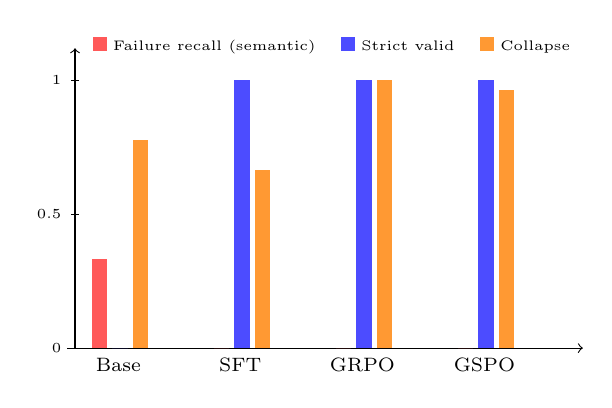
\begin{tikzpicture}[x=1cm,y=3.4cm]
\draw[->] (0.35,0) -- (6.9,0);
\draw[->] (0.45,0) -- (0.45,1.12);
\foreach \y in {0,0.5,1} {\draw (0.40,\y) -- (0.50,\y); \node[left,font=\tiny] at (0.40,\y) {\y};}

\fill[red!65] (0.66,0) rectangle (0.86,0.3333);
\fill[blue!70] (0.92,0) rectangle (1.12,0.0000);
\fill[orange!80] (1.18,0) rectangle (1.38,0.7778);
\node[below,font=\scriptsize] at (1.00,0) {Base};
\fill[red!65] (2.21,0) rectangle (2.41,0.0000);
\fill[blue!70] (2.47,0) rectangle (2.67,1.0000);
\fill[orange!80] (2.73,0) rectangle (2.93,0.6667);
\node[below,font=\scriptsize] at (2.55,0) {SFT};
\fill[red!65] (3.76,0) rectangle (3.96,0.0000);
\fill[blue!70] (4.02,0) rectangle (4.22,1.0000);
\fill[orange!80] (4.28,0) rectangle (4.48,1.0000);
\node[below,font=\scriptsize] at (4.10,0) {GRPO};
\fill[red!65] (5.31,0) rectangle (5.51,0.0000);
\fill[blue!70] (5.57,0) rectangle (5.77,1.0000);
\fill[orange!80] (5.83,0) rectangle (6.03,0.9630);
\node[below,font=\scriptsize] at (5.65,0) {GSPO};
\node[font=\tiny,anchor=west] at (0.55,1.13) {\textcolor{red!65}{\rule{5pt}{5pt}} Failure recall (semantic) \quad \textcolor{blue!70}{\rule{5pt}{5pt}} Strict valid \quad \textcolor{orange!80}{\rule{5pt}{5pt}} Collapse};
\end{tikzpicture}
}
\caption{V1 semantic failure recall, strict JSON validity, and collapse ratio. Historical discovery runs, not matched interventions.}
\label{fig:progression}
\end{figure}

\begin{figure}[t]
\centering
\resizebox{\columnwidth}{!}{% Generated from frozen V1 semantic state predictions.
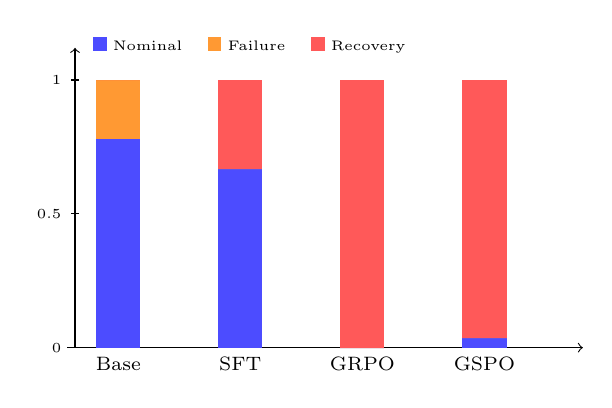
\begin{tikzpicture}[x=1cm,y=3.4cm]
\draw[->] (0.35,0) -- (6.9,0);
\draw[->] (0.45,0) -- (0.45,1.12);
\foreach \y in {0,0.5,1} {\draw (0.40,\y) -- (0.50,\y); \node[left,font=\tiny] at (0.40,\y) {\y};}

\fill[blue!70] (0.72,0.0000) rectangle (1.28,0.7778);
\fill[orange!80] (0.72,0.7778) rectangle (1.28,1.0000);
\fill[red!65] (0.72,1.0000) rectangle (1.28,1.0000);
\node[below,font=\scriptsize] at (1.00,0) {Base};
\fill[blue!70] (2.27,0.0000) rectangle (2.83,0.6667);
\fill[orange!80] (2.27,0.6667) rectangle (2.83,0.6667);
\fill[red!65] (2.27,0.6667) rectangle (2.83,1.0000);
\node[below,font=\scriptsize] at (2.55,0) {SFT};
\fill[blue!70] (3.82,0.0000) rectangle (4.38,0.0000);
\fill[orange!80] (3.82,0.0000) rectangle (4.38,0.0000);
\fill[red!65] (3.82,0.0000) rectangle (4.38,1.0000);
\node[below,font=\scriptsize] at (4.10,0) {GRPO};
\fill[blue!70] (5.37,0.0000) rectangle (5.93,0.0370);
\fill[orange!80] (5.37,0.0370) rectangle (5.93,0.0370);
\fill[red!65] (5.37,0.0370) rectangle (5.93,1.0000);
\node[below,font=\scriptsize] at (5.65,0) {GSPO};
\node[font=\tiny,anchor=west] at (0.55,1.13) {\textcolor{blue!70}{\rule{5pt}{5pt}} Nominal \quad \textcolor{orange!80}{\rule{5pt}{5pt}} Failure \quad \textcolor{red!65}{\rule{5pt}{5pt}} Recovery};
\end{tikzpicture}
}
\caption{Predicted state distributions after the fixed semantic parser. Base: 42 nominal/12 failure/0 recovery; SFT: 36/0/18; GRPO: 0/0/54; GSPO: 2/0/52.}
\label{fig:distribution}
\end{figure}

\section{Mechanism Isolation in V2}
We first remove phase and failure-mode outputs, training a critic with only a state field. Three matched two-camera views test observability: high+low, left+right wrist, and high+left wrist. We then compare sparse anchors with denser causal supervision on the validation-selected camera, holding the optimizer update budget fixed. Dense windows alter the class-frequency distribution; this is reported as a joint density/class-balance intervention unless a balancing control disentangles them. Finally, we compare separately trained visual-only and visual-plus-14-D-state/14-D-action Trace-Text models. Appending trace only at inference would be distribution shift and is excluded as a fair ablation.

Only if state-only validation predicts failure on at least two episodes do we test output-task interference: the same image input, episode split, seed, and update budget for a state-only versus phase/state/failure-mode adapter. Camera selection ranks validation failure recall, then State Macro-F1, with a fixed tie order; high recall can still arise from an all-failure predictor, so precision, false alarms, and class distribution remain essential. Table~\ref{tab:cameras} reports the completed validation screen. C2 wins the fixed rule with 15/15 failure windows recognized, but its 39.5\% failure precision and zero recovery recall do not support robust three-state monitoring; its Base control already recognized 15/15 failures by labeling 42/43 windows as failure. Strict JSON validity rises from 0/43 to 43/43 without changing failure recall. The V1 diagnostic score of the C2 SFT is not used for camera selection.

\begin{table}[t]
\centering\scriptsize
\resizebox{\columnwidth}{!}{% Generated from V2 validation metrics, not final-test results.
\begin{tabular}{lrrrrr}
\toprule
View & Base F-rec & SFT F-rec & SFT F-prec & SFT State F1 & SFT R-rec \\
\midrule
C0 & 100.0 & 80.0 & 35.3 & 31.5 & 0.0 \\
C1 & 73.3 & 46.7 & 36.8 & 44.7 & 33.3 \\
C2 & 100.0 & 100.0 & 39.5 & 30.0 & 0.0 \\
\bottomrule
\end{tabular}
}
\caption{V2 camera screen on the same five development-validation episodes. F-rec/F-prec are failure recall/precision; R-rec is recovery recall. Values are percentages; this is not the final refit test.}
\label{tab:cameras}
\end{table}

\section{Controlled Reward Intervention}
The historical additive verifier is
\begin{equation}
R_{\mathrm{add}}=0.25R_{\mathrm{phase}}+0.35R_{\mathrm{state}}+0.40R_{\mathrm{mode}}.
\end{equation}
Correct phase or mode can give positive reward despite a wrong execution state. Our state-gated verifier instead gives zero to invalid JSON, $-1$ to a missed true failure, zero to other wrong states, and $0.7+0.1R_{\mathrm{phase}}+0.2R_{\mathrm{mode}}$ only after the state is correct. This structure is validated with explicit wrong-state cases. Both controlled GRPO arms, if permitted, start from one SFT checkpoint and differ only in reward formulation; class reweighting is disabled in the additive arm. GRPO uses token-level importance ratios \cite{deepseekmath2024}; GSPO uses sequence-level ratios \cite{gspo2025} and is not automatically run.

The formal RL gate requires at least one more correctly detected validation failure window than matched Base, no State Macro-F1 regression or greater pre-failure false-alarm rate, at least 95\% strict JSON validity, residual failure-detection headroom, and a verified structured reward. If it fails, the RL outcome is \emph{not run}; V1 RL remains mechanism-discovery evidence only.

\section{Limitations and Status}
This is a small workshop study of a critic, not a recovery controller or production safety system. The V1 diagnostic set has six episodes and cannot yield a general cross-task claim. The state labels are annotation-grounded intervals, not independent human judgments of visual identifiability. A new single-task split, if used, is freshly frozen and its models retrained, but its episode pool overlaps the method-development pool; therefore it is weaker than a truly new task. FailBench already reports failure-detector fine-tuning regressions \cite{failbench2026}, while RoboMonitor reports effective temporal SFT \cite{robomonitor2026}; any final conclusion must be recipe- and evidence-specific. The V2 results, controlled RL gate, and final-test statistics will be inserted only from completed, machine-readable runs.

\bibliographystyle{unsrt}
\bibliography{references}
\end{document}
